% Requires: graphicx, booktabs, longtable, and subcaption.
\subsubsection{Benchmarking Predefined Text Categories}
\label{sec:cdp_text_classification}

We benchmark the classification of CDP text before applying a model to the 2016--2025 panel. The benchmark uses disclosures from 2020--2022 because these years provide a common questionnaire structure and manually validated observations. The full extracted datasets supply the underlying text, but predictive performance can be measured only for observations coded in the validation workbook. The evaluation sample contains 62 reduction items, 51 risk items, 181 opportunity items and 160 engagement items.

The task is classification rather than topic discovery. Each text item is assigned to a category defined before model estimation. Reduction items are classified by action family, such as renewable electricity, building energy efficiency, or transport and mobility. Risk and opportunity labels are consolidated into common types that can be applied across years. Engagement items are classified as engagement, policy, monitoring, response, or context. We also retain explicit negative categories, such as ``not a risk item'' and ``not an opportunity item.'' A separate ``other or unspecified'' category is available when a passage describes a core item but does not provide enough information for a substantive type. This distinction prevents responses and contextual statements from being treated as substantive risks or opportunities, while allowing genuinely new or poorly specified items to remain in the data.

We compare seven multilingual sentence encoders: MiniLM, E5-base, BGE-M3, Qwen3-Embedding-0.6B, GTE-multilingual, Jina-v3 and E5-large-instruct. An encoder converts a passage into a numeric vector that represents its meaning. For each encoder and disclosure section, a weighted multinomial logistic regression maps these vectors to the predefined categories. Class weights give relatively more importance to categories with few observations.

We use five-fold company-grouped cross-validation. All observations from a company are placed in the same fold, so the model is never evaluated on a company that it observed during training. Each model is trained on four folds and tested on the remaining fold; this process is repeated until every observation has an out-of-sample prediction. The procedure therefore evaluates classification of previously unseen companies rather than memorisation of company language.

We report accuracy, macro precision, macro recall and macro F1. Accuracy is the proportion of observations assigned the correct label. Precision measures how often predictions of a category are correct, while recall measures how many validated observations in that category are recovered. F1 is the harmonic mean of precision and recall. The macro measures first calculate the score for each category and then give every category equal weight. Macro F1 is consequently the primary criterion because accuracy can be high when a model predicts a large category well but fails on smaller categories. The output also reports weighted F1, balanced accuracy, the Matthews correlation coefficient and whether each test label appeared in its corresponding training fold.

\begin{figure}[!htbp]
    \centering
    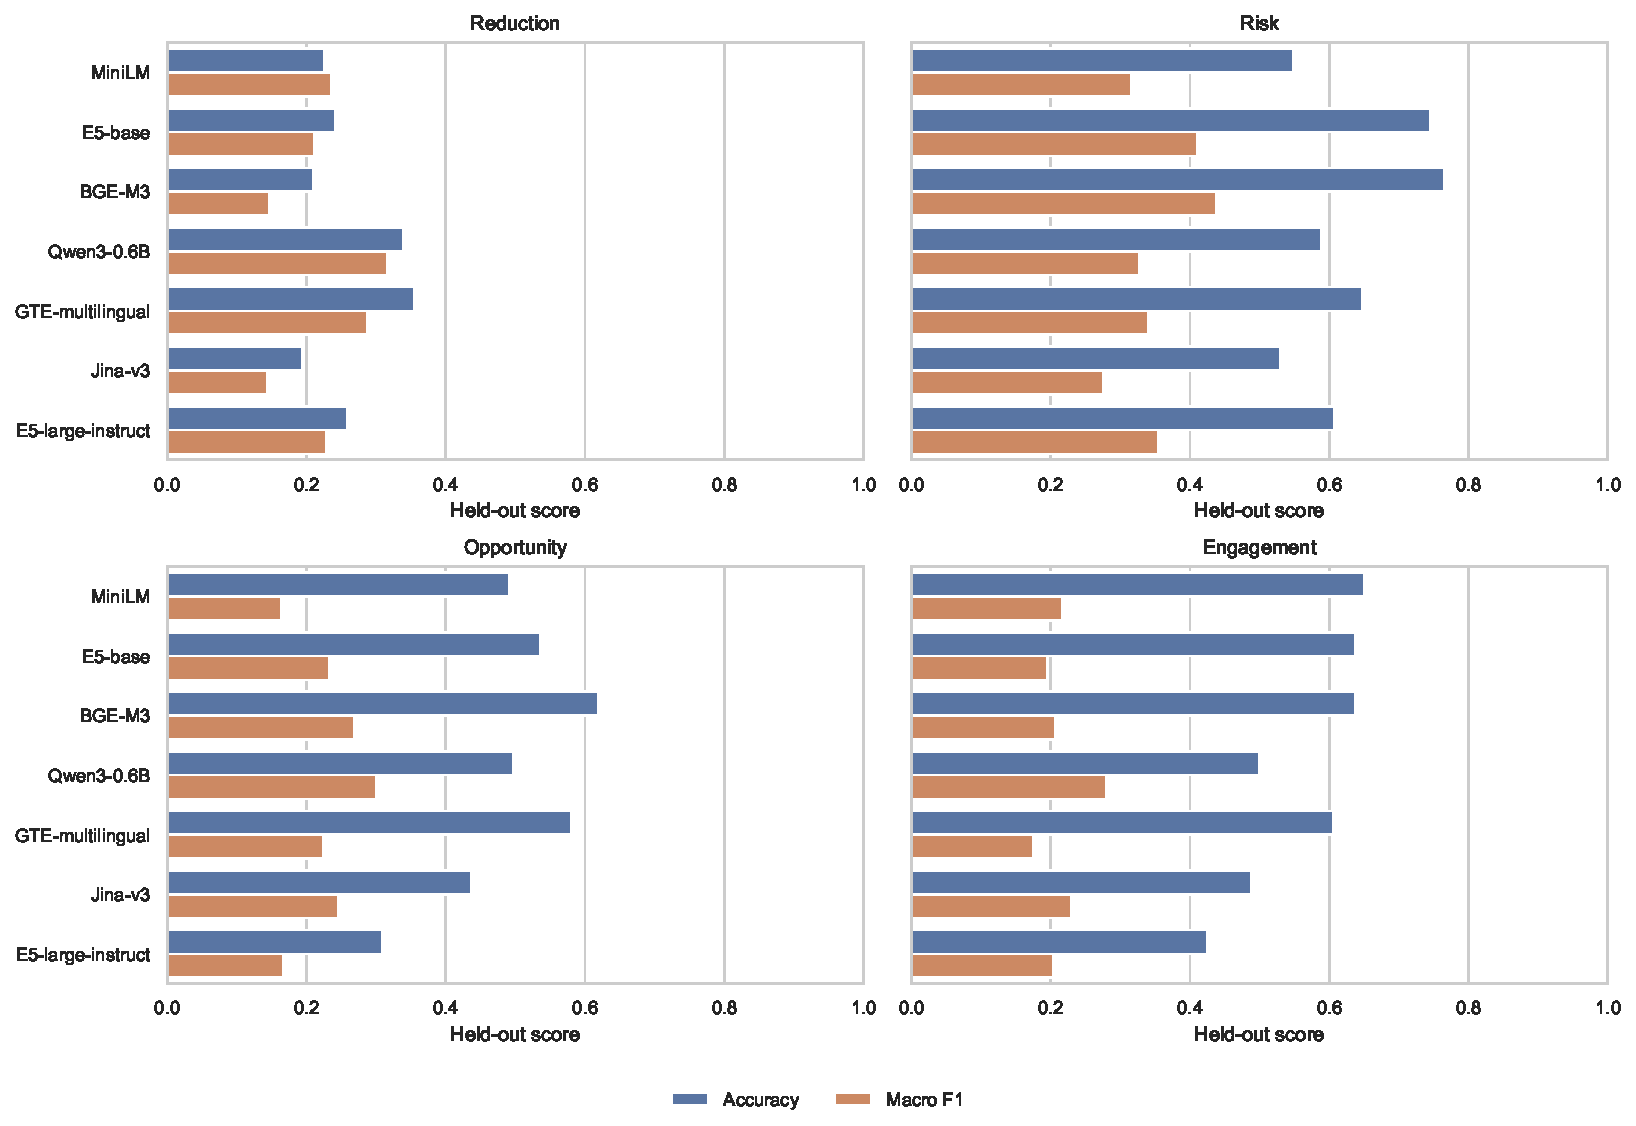
\includegraphics[width=\linewidth]{reports/cdp_text_clustering/cdp_defined_action_taxonomy_2020_2022/model_accuracy_macro_f1.pdf}
    \caption{Out-of-Sample Accuracy and Macro F1 by Encoder and Disclosure Section}
    \label{fig:cdp_model_accuracy_f1}
    \begin{minipage}{\linewidth}\footnotesize
        \textit{Notes.} Results use five-fold company-grouped cross-validation on validated 2020--2022 items. Accuracy weights observations equally; macro F1 weights categories equally. Differences between these measures indicate class imbalance.
    \end{minipage}
\end{figure}

\begin{longtable}{llrrrrrr}
\caption{Company-grouped classification performance by encoder and disclosure section.} \label{tab:cdp_text_classification_models} \\
\toprule
model & section & observations & classes & accuracy & macro\_precision & macro\_recall & macro\_f1 \\
\midrule
\endfirsthead
\caption[]{Company-grouped classification performance by encoder and disclosure section.} \\
\toprule
model & section & observations & classes & accuracy & macro\_precision & macro\_recall & macro\_f1 \\
\midrule
\endhead
\midrule
\multicolumn{8}{r}{Continued on next page} \\
\midrule
\endfoot
\bottomrule
\endlastfoot
MiniLM & reduction & 62 & 11 & 0.226 & 0.268 & 0.256 & 0.236 \\
MiniLM & risk & 51 & 7 & 0.549 & 0.316 & 0.320 & 0.316 \\
MiniLM & opportunity & 181 & 6 & 0.492 & 0.179 & 0.171 & 0.165 \\
MiniLM & engagement & 160 & 5 & 0.650 & 0.215 & 0.219 & 0.217 \\
E5-base & reduction & 62 & 11 & 0.242 & 0.196 & 0.238 & 0.212 \\
E5-base & risk & 51 & 7 & 0.745 & 0.386 & 0.442 & 0.411 \\
E5-base & opportunity & 181 & 6 & 0.536 & 0.253 & 0.232 & 0.233 \\
E5-base & engagement & 160 & 5 & 0.637 & 0.193 & 0.199 & 0.195 \\
BGE-M3 & reduction & 62 & 11 & 0.210 & 0.121 & 0.189 & 0.147 \\
BGE-M3 & risk & 51 & 7 & 0.765 & 0.448 & 0.450 & 0.438 \\
BGE-M3 & opportunity & 181 & 6 & 0.619 & 0.349 & 0.248 & 0.269 \\
BGE-M3 & engagement & 160 & 5 & 0.637 & 0.201 & 0.215 & 0.207 \\
Qwen3-0.6B & reduction & 62 & 11 & 0.339 & 0.345 & 0.316 & 0.317 \\
Qwen3-0.6B & risk & 51 & 7 & 0.588 & 0.316 & 0.361 & 0.327 \\
Qwen3-0.6B & opportunity & 181 & 6 & 0.497 & 0.273 & 0.399 & 0.300 \\
Qwen3-0.6B & engagement & 160 & 5 & 0.500 & 0.293 & 0.292 & 0.280 \\
GTE-multilingual & reduction & 62 & 11 & 0.355 & 0.248 & 0.350 & 0.287 \\
GTE-multilingual & risk & 51 & 7 & 0.647 & 0.338 & 0.362 & 0.340 \\
GTE-multilingual & opportunity & 181 & 6 & 0.580 & 0.223 & 0.244 & 0.225 \\
GTE-multilingual & engagement & 160 & 5 & 0.606 & 0.176 & 0.176 & 0.175 \\
Jina-v3 & reduction & 62 & 11 & 0.194 & 0.131 & 0.167 & 0.143 \\
Jina-v3 & risk & 51 & 7 & 0.529 & 0.262 & 0.311 & 0.276 \\
Jina-v3 & opportunity & 181 & 6 & 0.436 & 0.244 & 0.335 & 0.246 \\
Jina-v3 & engagement & 160 & 5 & 0.487 & 0.230 & 0.272 & 0.230 \\
E5-large-instruct & reduction & 62 & 11 & 0.258 & 0.237 & 0.266 & 0.228 \\
E5-large-instruct & risk & 51 & 7 & 0.608 & 0.332 & 0.432 & 0.355 \\
E5-large-instruct & opportunity & 181 & 6 & 0.309 & 0.184 & 0.231 & 0.167 \\
E5-large-instruct & engagement & 160 & 5 & 0.425 & 0.223 & 0.238 & 0.204 \\
\end{longtable}


Qwen3-0.6B obtains the highest mean macro F1 across the four sections (0.306), followed by BGE-M3 (0.265) and E5-base (0.263). Its section-level macro F1 values are 0.317 for reduction actions, 0.327 for risks, 0.300 for opportunities and 0.280 for engagement. Its corresponding accuracies are 0.339, 0.588, 0.497 and 0.500. BGE-M3 has the highest mean accuracy (0.558), including an accuracy of 0.765 and macro F1 of 0.438 for risks. This difference shows why accuracy alone is not sufficient: BGE-M3 performs well on common labels, whereas Qwen3-0.6B is more balanced across sections and categories.

The confusion matrices in Figures~\ref{fig:cdp_confusion_reduction}--\ref{fig:cdp_confusion_engagement} show where Qwen3-0.6B succeeds and fails. For example, it identifies renewable electricity and transport actions more reliably than planning, monitoring, or materials-related actions. It also identifies acute physical risks well, but performance is weak for chronic physical, market, and technology risks because these categories have few validated observations. In the opportunity sample, the large ``not an opportunity item'' category is substantially easier to identify than the smaller substantive categories. Monitoring is similarly underrepresented in the engagement sample.

We separately inspect initiative records that the current taxonomy leaves unclassified. This review distinguishes missing classifications from potential new concepts. Of 539 unclassified initiatives in the extracted 2020--2022 data, text rules identify 72 as members of existing families, including transport and mobility, credits and neutralisation, fuel substitution, products and materials, and operational energy efficiency. Twenty-three records support two candidate additions: nature and land-use interventions (15 records) and water-efficiency interventions (8 records). These candidates are not added automatically because their small counts and possible overlap require manual validation. The remaining 444 records either lack a supported label or match several candidates and are retained for review. This procedure prevents a residual category from becoming a collection of unrelated activities.

\begin{figure}[!htbp]
    \centering
    \begin{subfigure}[t]{0.49\linewidth}
        \centering
        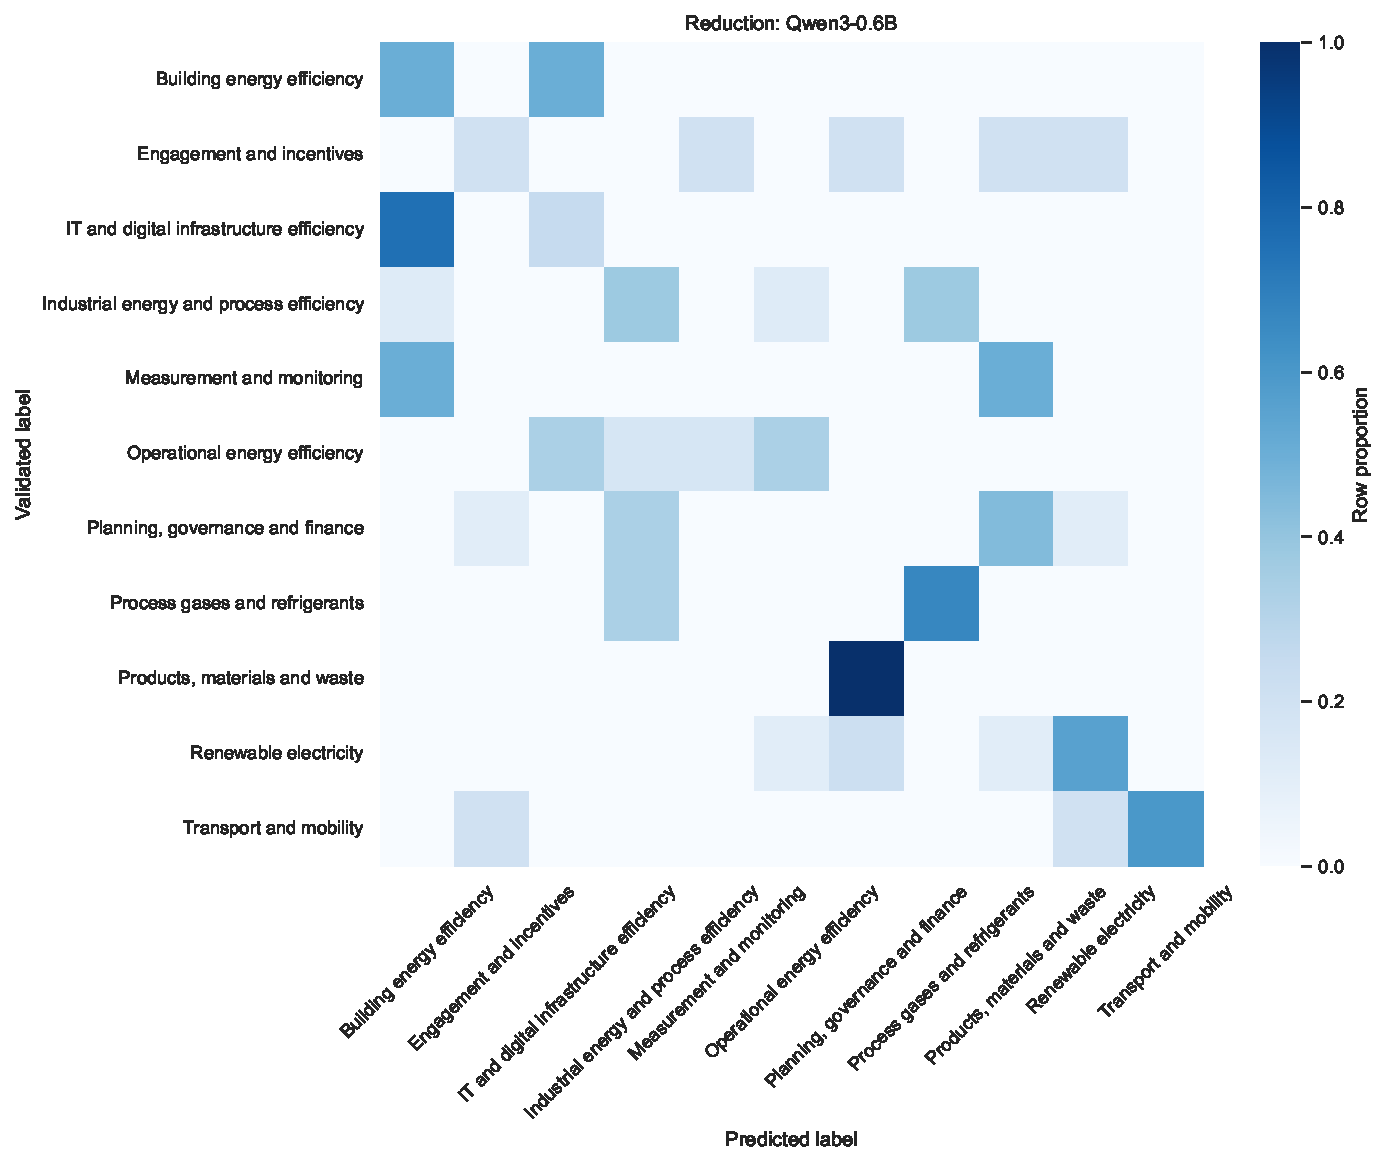
\includegraphics[width=\linewidth]{reports/cdp_text_clustering/cdp_defined_action_taxonomy_2020_2022/confusion_reduction_qwen3_06b.pdf}
        \caption{Reduction actions}
        \label{fig:cdp_confusion_reduction}
    \end{subfigure}
    \hfill
    \begin{subfigure}[t]{0.49\linewidth}
        \centering
        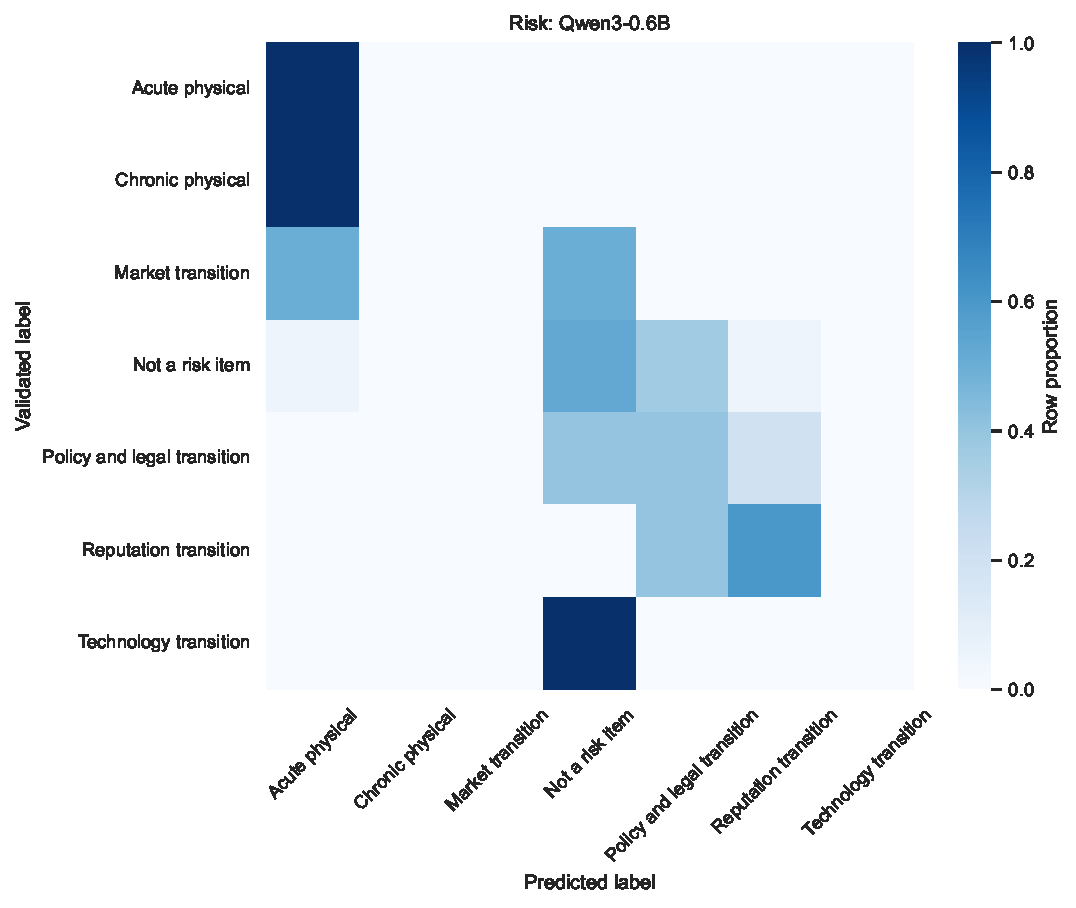
\includegraphics[width=\linewidth]{reports/cdp_text_clustering/cdp_defined_action_taxonomy_2020_2022/confusion_risk_qwen3_06b.pdf}
        \caption{Risks}
        \label{fig:cdp_confusion_risk}
    \end{subfigure}
    \par\medskip
    \begin{subfigure}[t]{0.49\linewidth}
        \centering
        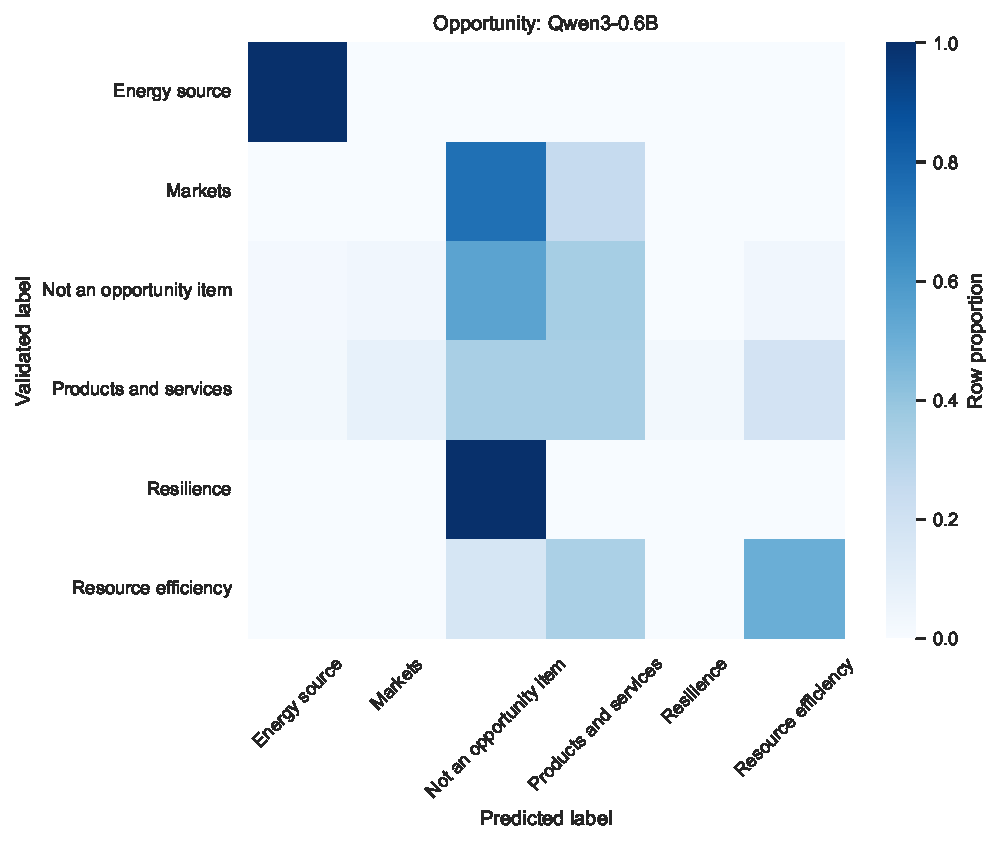
\includegraphics[width=\linewidth]{reports/cdp_text_clustering/cdp_defined_action_taxonomy_2020_2022/confusion_opportunity_qwen3_06b.pdf}
        \caption{Opportunities}
        \label{fig:cdp_confusion_opportunity}
    \end{subfigure}
    \hfill
    \begin{subfigure}[t]{0.49\linewidth}
        \centering
        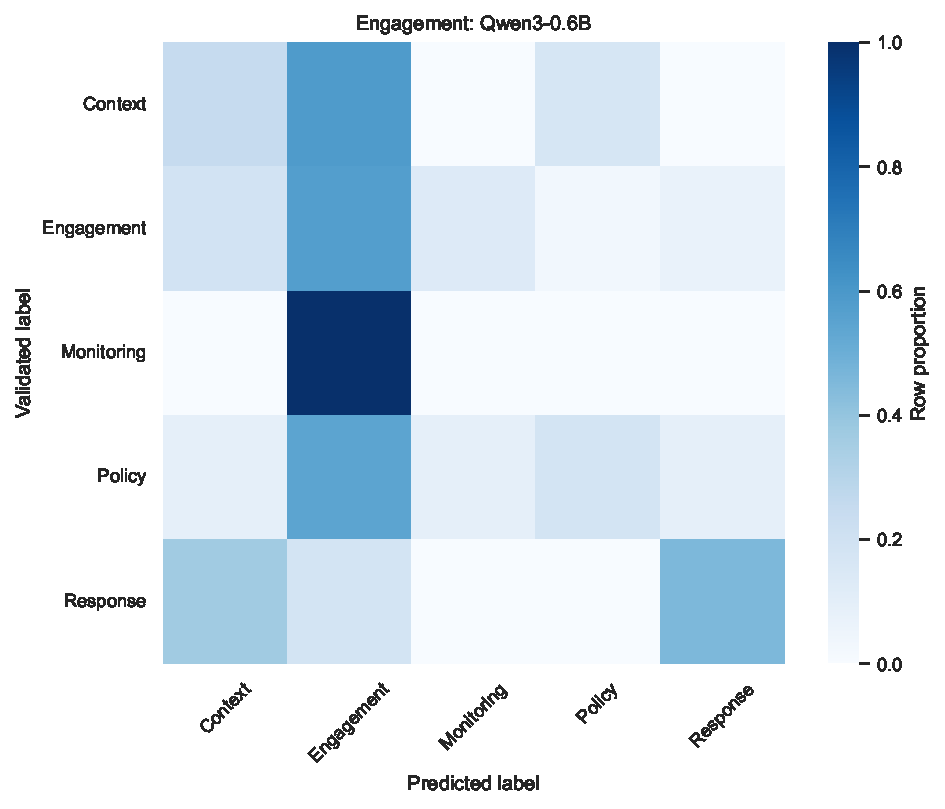
\includegraphics[width=\linewidth]{reports/cdp_text_clustering/cdp_defined_action_taxonomy_2020_2022/confusion_engagement_qwen3_06b.pdf}
        \caption{Engagement}
        \label{fig:cdp_confusion_engagement}
    \end{subfigure}
    \caption{Normalised Confusion Matrices for Qwen3-0.6B}
    \begin{minipage}{\linewidth}\footnotesize
        \textit{Notes.} Rows are validated categories and columns are predicted categories. Each row sums to one. Dark diagonal cells indicate correct classification; off-diagonal cells show the categories that the model confuses.
    \end{minipage}
\end{figure}

The benchmark does not yet support unreviewed application to the complete 2016--2025 dataset. The best mean macro F1 remains 0.306, and several rare categories have zero recall. Qwen3-0.6B is the strongest single-model candidate under the prespecified macro-F1 criterion, while BGE-M3 is the strongest risk classifier in this sample. Before final deployment, we will review errors, add validated examples for poorly represented categories and test whether a section-specific choice---BGE-M3 for risks and Qwen3-0.6B for the other sections---improves performance on a separate verification sample. The final model will then classify the 2016--2025 data, with low-confidence and other-or-unspecified predictions retained for manual review rather than assigned to a substantive category automatically.
